\documentclass[twoside]{book}

% Packages required by doxygen
\usepackage{fixltx2e}
\usepackage{calc}
\usepackage{doxygen}
\usepackage[export]{adjustbox} % also loads graphicx
\usepackage{graphicx}
\usepackage[utf8]{inputenc}
\usepackage{makeidx}
\usepackage{multicol}
\usepackage{multirow}
\PassOptionsToPackage{warn}{textcomp}
\usepackage{textcomp}
\usepackage[nointegrals]{wasysym}
\usepackage[table]{xcolor}

% Font selection
\usepackage[T1]{fontenc}
\usepackage[scaled=.90]{helvet}
\usepackage{courier}
\usepackage{amssymb}
\usepackage{sectsty}
\renewcommand{\familydefault}{\sfdefault}
\allsectionsfont{%
  \fontseries{bc}\selectfont%
  \color{darkgray}%
}
\renewcommand{\DoxyLabelFont}{%
  \fontseries{bc}\selectfont%
  \color{darkgray}%
}
\newcommand{\+}{\discretionary{\mbox{\scriptsize$\hookleftarrow$}}{}{}}

% Page & text layout
\usepackage{geometry}
\geometry{%
  a4paper,%
  top=2.5cm,%
  bottom=2.5cm,%
  left=2.5cm,%
  right=2.5cm%
}
\tolerance=750
\hfuzz=15pt
\hbadness=750
\setlength{\emergencystretch}{15pt}
\setlength{\parindent}{0cm}
\setlength{\parskip}{0.2cm}
\makeatletter
\renewcommand{\paragraph}{%
  \@startsection{paragraph}{4}{0ex}{-1.0ex}{1.0ex}{%
    \normalfont\normalsize\bfseries\SS@parafont%
  }%
}
\renewcommand{\subparagraph}{%
  \@startsection{subparagraph}{5}{0ex}{-1.0ex}{1.0ex}{%
    \normalfont\normalsize\bfseries\SS@subparafont%
  }%
}
\makeatother

% Headers & footers
\usepackage{fancyhdr}
\pagestyle{fancyplain}
\fancyhead[LE]{\fancyplain{}{\bfseries\thepage}}
\fancyhead[CE]{\fancyplain{}{}}
\fancyhead[RE]{\fancyplain{}{\bfseries\leftmark}}
\fancyhead[LO]{\fancyplain{}{\bfseries\rightmark}}
\fancyhead[CO]{\fancyplain{}{}}
\fancyhead[RO]{\fancyplain{}{\bfseries\thepage}}
\fancyfoot[LE]{\fancyplain{}{}}
\fancyfoot[CE]{\fancyplain{}{}}
\fancyfoot[RE]{\fancyplain{}{\bfseries\scriptsize Generated on Sun Jan 25 2015 19\+:18\+:40 for Lib\+Fleaux by Doxygen }}
\fancyfoot[LO]{\fancyplain{}{\bfseries\scriptsize Generated on Sun Jan 25 2015 19\+:18\+:40 for Lib\+Fleaux by Doxygen }}
\fancyfoot[CO]{\fancyplain{}{}}
\fancyfoot[RO]{\fancyplain{}{}}
\renewcommand{\footrulewidth}{0.4pt}
\renewcommand{\chaptermark}[1]{%
  \markboth{#1}{}%
}
\renewcommand{\sectionmark}[1]{%
  \markright{\thesection\ #1}%
}

% Indices & bibliography
\usepackage{natbib}
\usepackage[titles]{tocloft}
\setcounter{tocdepth}{3}
\setcounter{secnumdepth}{5}
\makeindex

% Hyperlinks (required, but should be loaded last)
\usepackage{ifpdf}
\ifpdf
  \usepackage[pdftex,pagebackref=true]{hyperref}
\else
  \usepackage[ps2pdf,pagebackref=true]{hyperref}
\fi
\hypersetup{%
  colorlinks=true,%
  linkcolor=blue,%
  citecolor=blue,%
  unicode%
}

% Custom commands
\newcommand{\clearemptydoublepage}{%
  \newpage{\pagestyle{empty}\cleardoublepage}%
}


%===== C O N T E N T S =====

\begin{document}

% Titlepage & ToC
\hypersetup{pageanchor=false,
             bookmarks=true,
             bookmarksnumbered=true,
             pdfencoding=unicode
            }
\pagenumbering{roman}
\begin{titlepage}
\vspace*{7cm}
\begin{center}%
{\Large Lib\+Fleaux \\[1ex]\large 0.\+0.\+0 }\\
\vspace*{1cm}
{\large Generated by Doxygen 1.8.9.1}\\
\vspace*{0.5cm}
{\small Sun Jan 25 2015 19:18:40}\\
\end{center}
\end{titlepage}
\clearemptydoublepage
\tableofcontents
\clearemptydoublepage
\pagenumbering{arabic}
\hypersetup{pageanchor=true}

%--- Begin generated contents ---
\chapter{Hierarchical Index}
\section{Class Hierarchy}
This inheritance list is sorted roughly, but not completely, alphabetically\+:\begin{DoxyCompactList}
\item \contentsline{section}{Fleaux\+:\+:I\+Cursor}{\pageref{classFleaux_1_1ICursor}}{}
\begin{DoxyCompactList}
\item \contentsline{section}{Fleaux\+:\+:Cursor}{\pageref{classFleaux_1_1Cursor}}{}
\end{DoxyCompactList}
\item \contentsline{section}{Fleaux\+:\+:I\+Editor}{\pageref{classFleaux_1_1IEditor}}{}
\begin{DoxyCompactList}
\item \contentsline{section}{Fleaux\+:\+:Editor}{\pageref{classFleaux_1_1Editor}}{}
\end{DoxyCompactList}
\end{DoxyCompactList}

\chapter{Class Index}
\section{Class List}
Here are the classes, structs, unions and interfaces with brief descriptions\+:\begin{DoxyCompactList}
\item\contentsline{section}{\hyperlink{classFleaux_1_1Cursor}{Fleaux\+::\+Cursor} }{\pageref{classFleaux_1_1Cursor}}{}
\item\contentsline{section}{\hyperlink{classFleaux_1_1Editor}{Fleaux\+::\+Editor} }{\pageref{classFleaux_1_1Editor}}{}
\end{DoxyCompactList}

\chapter{Class Documentation}
\hypertarget{classFleaux_1_1Cursor}{}\section{Fleaux\+:\+:Cursor Class Reference}
\label{classFleaux_1_1Cursor}\index{Fleaux\+::\+Cursor@{Fleaux\+::\+Cursor}}
Inheritance diagram for Fleaux\+:\+:Cursor\+:\begin{figure}[H]
\begin{center}
\leavevmode
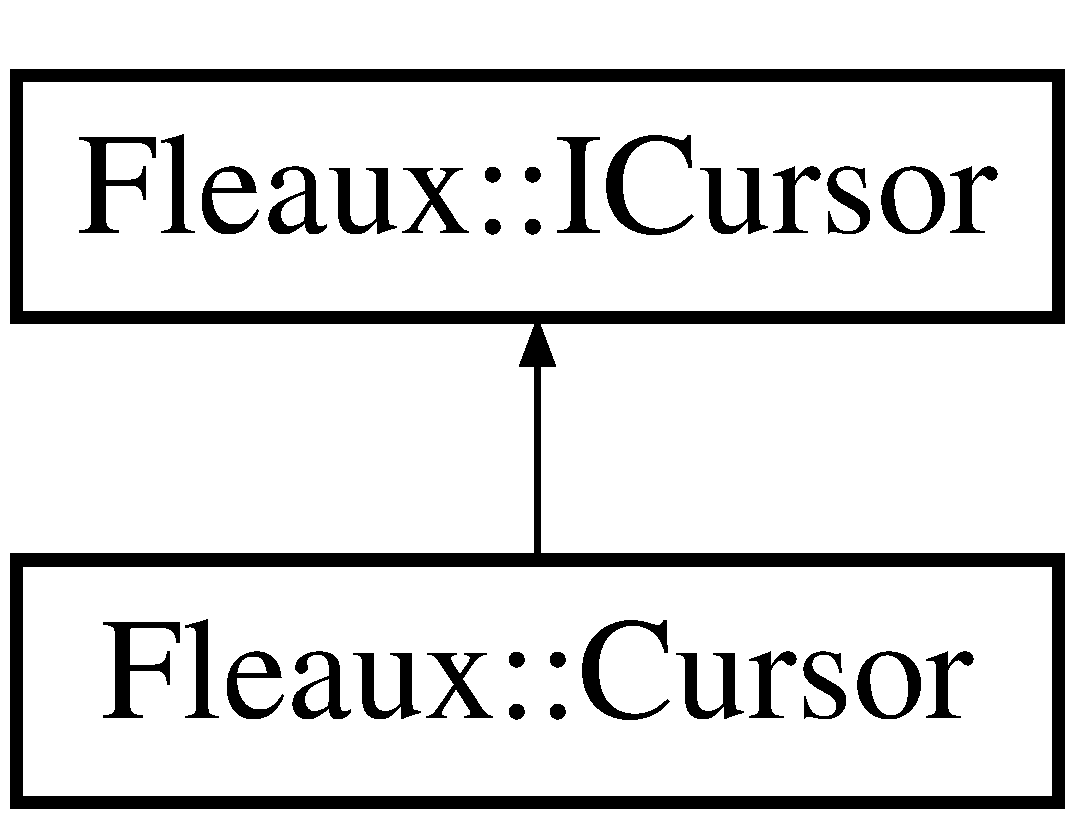
\includegraphics[height=2.000000cm]{classFleaux_1_1Cursor}
\end{center}
\end{figure}
\subsection*{Public Member Functions}
\begin{DoxyCompactItemize}
\item 
\hyperlink{classFleaux_1_1Cursor_aa2811c8ebadd1b019a1d1099eb401e3b}{Cursor} (\hyperlink{classFleaux_1_1Editor}{Editor} $\ast$ed)
\item 
\hyperlink{classFleaux_1_1Cursor_a643ea893489f5a963473dc79afd65bd2}{Cursor} (const \hyperlink{classFleaux_1_1ICursor}{I\+Cursor} \&curs)
\item 
void \hyperlink{classFleaux_1_1Cursor_a99c820ad3d952b5e38a41a11c18e7c2f}{insert} (const string \&input)
\item 
void \hyperlink{classFleaux_1_1Cursor_a0fca52d6d4e589f8eef50a351e8340ff}{remove} (int length)
\item 
void \hyperlink{classFleaux_1_1Cursor_a439606f718dd885f4f96ca3244c3172a}{replace} (int length, const string \&replacement)
\item 
\hypertarget{classFleaux_1_1Cursor_a9cdba74fcd1c812bdfd97b671fbef659}{}\hyperlink{classFleaux_1_1IEditor}{I\+Editor} $\ast$ {\bfseries get\+Editor} (void) const \label{classFleaux_1_1Cursor_a9cdba74fcd1c812bdfd97b671fbef659}

\item 
\hypertarget{classFleaux_1_1Cursor_a7358d0be48db3117802279959c125eb8}{}size\+\_\+t {\bfseries get\+Index} (void) const \label{classFleaux_1_1Cursor_a7358d0be48db3117802279959c125eb8}

\item 
\hypertarget{classFleaux_1_1Cursor_a3dc9befeb121b6a536da063560f81af0}{}size\+\_\+t {\bfseries get\+X} (void) const \label{classFleaux_1_1Cursor_a3dc9befeb121b6a536da063560f81af0}

\item 
\hypertarget{classFleaux_1_1Cursor_ab265ba6839087cbe810c27fe59e9f593}{}size\+\_\+t {\bfseries get\+Y} (void) const \label{classFleaux_1_1Cursor_ab265ba6839087cbe810c27fe59e9f593}

\item 
void \hyperlink{classFleaux_1_1Cursor_a91e3ff97154764836099fdb13002c877}{move} (int offset\+X, int offset\+Y)
\end{DoxyCompactItemize}
\subsection*{Protected Member Functions}
\begin{DoxyCompactItemize}
\item 
void \hyperlink{classFleaux_1_1Cursor_a3a45b2bde24c3173e84b8097c789265b}{\+\_\+set\+X\+Y} (void)
\item 
void \hyperlink{classFleaux_1_1Cursor_a964ad98494b190af5fca13c8cbe69371}{\+\_\+set\+Index} (void)
\end{DoxyCompactItemize}
\subsection*{Protected Attributes}
\begin{DoxyCompactItemize}
\item 
\hypertarget{classFleaux_1_1Cursor_ac73c77f866d9fd3ce6ac74f458f899b5}{}size\+\_\+t {\bfseries \+\_\+index}\label{classFleaux_1_1Cursor_ac73c77f866d9fd3ce6ac74f458f899b5}

\item 
\hypertarget{classFleaux_1_1Cursor_acbb4e71f0e8fe82c57d4046d708e94c8}{}size\+\_\+t {\bfseries \+\_\+x}\label{classFleaux_1_1Cursor_acbb4e71f0e8fe82c57d4046d708e94c8}

\item 
\hypertarget{classFleaux_1_1Cursor_ae31481eee36242bfcb286fb03cb6c9d9}{}size\+\_\+t {\bfseries \+\_\+y}\label{classFleaux_1_1Cursor_ae31481eee36242bfcb286fb03cb6c9d9}

\item 
\hypertarget{classFleaux_1_1Cursor_ae65c902eba05392c7db5cb8956af441d}{}\hyperlink{classFleaux_1_1Editor}{Editor} $\ast$ {\bfseries \+\_\+editor}\label{classFleaux_1_1Cursor_ae65c902eba05392c7db5cb8956af441d}

\end{DoxyCompactItemize}


\subsection{Constructor \& Destructor Documentation}
\hypertarget{classFleaux_1_1Cursor_aa2811c8ebadd1b019a1d1099eb401e3b}{}\index{Fleaux\+::\+Cursor@{Fleaux\+::\+Cursor}!Cursor@{Cursor}}
\index{Cursor@{Cursor}!Fleaux\+::\+Cursor@{Fleaux\+::\+Cursor}}
\subsubsection[{Cursor}]{\setlength{\rightskip}{0pt plus 5cm}Fleaux\+::\+Cursor\+::\+Cursor (
\begin{DoxyParamCaption}
\item[{{\bf Editor} $\ast$}]{ed}
\end{DoxyParamCaption}
)}\label{classFleaux_1_1Cursor_aa2811c8ebadd1b019a1d1099eb401e3b}
Constructor creates a new \hyperlink{classFleaux_1_1Cursor}{Cursor} instance that belongs to the editor pointed to by ed. The optional caller\+Is\+Editor parameter is used to determine if this is being called from an \hyperlink{classFleaux_1_1Editor}{Editor}\textquotesingle{}s constructor, or by another entity. If the call is being made outside of an editor\textquotesingle{}s constructor, then the new cursor is merely a copy of ed\textquotesingle{}s \hypertarget{classFleaux_1_1Cursor_a643ea893489f5a963473dc79afd65bd2}{}\index{Fleaux\+::\+Cursor@{Fleaux\+::\+Cursor}!Cursor@{Cursor}}
\index{Cursor@{Cursor}!Fleaux\+::\+Cursor@{Fleaux\+::\+Cursor}}
\subsubsection[{Cursor}]{\setlength{\rightskip}{0pt plus 5cm}Fleaux\+::\+Cursor\+::\+Cursor (
\begin{DoxyParamCaption}
\item[{const {\bf I\+Cursor} \&}]{curs}
\end{DoxyParamCaption}
)}\label{classFleaux_1_1Cursor_a643ea893489f5a963473dc79afd65bd2}
Copy constructor -\/ Simple shallow copy. 

\subsection{Member Function Documentation}
\hypertarget{classFleaux_1_1Cursor_a964ad98494b190af5fca13c8cbe69371}{}\index{Fleaux\+::\+Cursor@{Fleaux\+::\+Cursor}!\+\_\+set\+Index@{\+\_\+set\+Index}}
\index{\+\_\+set\+Index@{\+\_\+set\+Index}!Fleaux\+::\+Cursor@{Fleaux\+::\+Cursor}}
\subsubsection[{\+\_\+set\+Index}]{\setlength{\rightskip}{0pt plus 5cm}void Fleaux\+::\+Cursor\+::\+\_\+set\+Index (
\begin{DoxyParamCaption}
\item[{void}]{}
\end{DoxyParamCaption}
)\hspace{0.3cm}{\ttfamily [protected]}}\label{classFleaux_1_1Cursor_a964ad98494b190af5fca13c8cbe69371}
Calculates the cursor\textquotesingle{}s new index after updating it\textquotesingle{}s x and/or y value(s). \hypertarget{classFleaux_1_1Cursor_a3a45b2bde24c3173e84b8097c789265b}{}\index{Fleaux\+::\+Cursor@{Fleaux\+::\+Cursor}!\+\_\+set\+X\+Y@{\+\_\+set\+X\+Y}}
\index{\+\_\+set\+X\+Y@{\+\_\+set\+X\+Y}!Fleaux\+::\+Cursor@{Fleaux\+::\+Cursor}}
\subsubsection[{\+\_\+set\+X\+Y}]{\setlength{\rightskip}{0pt plus 5cm}void Fleaux\+::\+Cursor\+::\+\_\+set\+X\+Y (
\begin{DoxyParamCaption}
\item[{void}]{}
\end{DoxyParamCaption}
)\hspace{0.3cm}{\ttfamily [protected]}}\label{classFleaux_1_1Cursor_a3a45b2bde24c3173e84b8097c789265b}
Calculates the cursor\textquotesingle{}s new x and/or y value(s) after updating its index. \hypertarget{classFleaux_1_1Cursor_a99c820ad3d952b5e38a41a11c18e7c2f}{}\index{Fleaux\+::\+Cursor@{Fleaux\+::\+Cursor}!insert@{insert}}
\index{insert@{insert}!Fleaux\+::\+Cursor@{Fleaux\+::\+Cursor}}
\subsubsection[{insert}]{\setlength{\rightskip}{0pt plus 5cm}void Fleaux\+::\+Cursor\+::insert (
\begin{DoxyParamCaption}
\item[{const string \&}]{input}
\end{DoxyParamCaption}
)\hspace{0.3cm}{\ttfamily [virtual]}}\label{classFleaux_1_1Cursor_a99c820ad3d952b5e38a41a11c18e7c2f}
Inserts the input string at the cursor\textquotesingle{}s current position in the editor\textquotesingle{}s buffer. 

Implements \hyperlink{classFleaux_1_1ICursor}{Fleaux\+::\+I\+Cursor}.

\hypertarget{classFleaux_1_1Cursor_a91e3ff97154764836099fdb13002c877}{}\index{Fleaux\+::\+Cursor@{Fleaux\+::\+Cursor}!move@{move}}
\index{move@{move}!Fleaux\+::\+Cursor@{Fleaux\+::\+Cursor}}
\subsubsection[{move}]{\setlength{\rightskip}{0pt plus 5cm}void Fleaux\+::\+Cursor\+::move (
\begin{DoxyParamCaption}
\item[{int}]{offset\+X, }
\item[{int}]{offset\+Y}
\end{DoxyParamCaption}
)\hspace{0.3cm}{\ttfamily [virtual]}}\label{classFleaux_1_1Cursor_a91e3ff97154764836099fdb13002c877}
Moves the cursor relative to its current x,y position. For example\+: calling move(-\/4, 27) will move the cursor left 4 characters and down 27 characters 

Implements \hyperlink{classFleaux_1_1ICursor}{Fleaux\+::\+I\+Cursor}.

\hypertarget{classFleaux_1_1Cursor_a0fca52d6d4e589f8eef50a351e8340ff}{}\index{Fleaux\+::\+Cursor@{Fleaux\+::\+Cursor}!remove@{remove}}
\index{remove@{remove}!Fleaux\+::\+Cursor@{Fleaux\+::\+Cursor}}
\subsubsection[{remove}]{\setlength{\rightskip}{0pt plus 5cm}void Fleaux\+::\+Cursor\+::remove (
\begin{DoxyParamCaption}
\item[{int}]{length}
\end{DoxyParamCaption}
)\hspace{0.3cm}{\ttfamily [virtual]}}\label{classFleaux_1_1Cursor_a0fca52d6d4e589f8eef50a351e8340ff}
Removes n characters, where n is $\vert$length$\vert$. The sign of length determines the direction from the cursor in which characters are removed\+: (-\/) removes backward starting at the character behind the cursor, (+) removes forward starting at the character under the cursor. 

Implements \hyperlink{classFleaux_1_1ICursor}{Fleaux\+::\+I\+Cursor}.

\hypertarget{classFleaux_1_1Cursor_a439606f718dd885f4f96ca3244c3172a}{}\index{Fleaux\+::\+Cursor@{Fleaux\+::\+Cursor}!replace@{replace}}
\index{replace@{replace}!Fleaux\+::\+Cursor@{Fleaux\+::\+Cursor}}
\subsubsection[{replace}]{\setlength{\rightskip}{0pt plus 5cm}void Fleaux\+::\+Cursor\+::replace (
\begin{DoxyParamCaption}
\item[{int}]{length, }
\item[{const string \&}]{replacement}
\end{DoxyParamCaption}
)\hspace{0.3cm}{\ttfamily [virtual]}}\label{classFleaux_1_1Cursor_a439606f718dd885f4f96ca3244c3172a}
Replaces n characters in where n is $\vert$length$\vert$ with the replacement string. This is the same as Fleaux\+::\+Cursor\+::remove(length) followed by Fleaux\+::\+Cursor\+::insert(replacement). 

Implements \hyperlink{classFleaux_1_1ICursor}{Fleaux\+::\+I\+Cursor}.



The documentation for this class was generated from the following files\+:\begin{DoxyCompactItemize}
\item 
src/fleaux/headers/editor.\+hh\item 
src/fleaux/cpp/editor.\+cc\end{DoxyCompactItemize}

\hypertarget{classFleaux_1_1Editor}{}\section{Fleaux\+:\+:Editor Class Reference}
\label{classFleaux_1_1Editor}\index{Fleaux\+::\+Editor@{Fleaux\+::\+Editor}}
\subsection*{Public Member Functions}
\begin{DoxyCompactItemize}
\item 
\hyperlink{classFleaux_1_1Editor_a5425124a3ddf55ad2fe2b668548c011f}{Editor} (void)
\item 
\hyperlink{classFleaux_1_1Editor_a023e2569b82e4299d02ddbd0a912fc5e}{Editor} (const string \&path)
\item 
\hyperlink{classFleaux_1_1Editor_a44125eb3c92f032db297029b0039eef8}{Editor} (const \hyperlink{classFleaux_1_1Editor}{Editor} \&ed)
\item 
\hyperlink{classFleaux_1_1Editor_a2be65be385e3a41d16c426c7bcdc00d9}{$\sim$\+Editor} (void)
\item 
void \hyperlink{classFleaux_1_1Editor_ac525cdc5632ff3cf1664a2088a4306e6}{read\+From\+File} (const string \&path)
\item 
void \hyperlink{classFleaux_1_1Editor_ad6f189d15112586cc5cefd37ab82e5f0}{write\+To\+File} (const string \&path)
\item 
\hypertarget{classFleaux_1_1Editor_a71402c284080c5e797086002ccec050e}{}size\+\_\+t {\bfseries get\+Size} (void) const \label{classFleaux_1_1Editor_a71402c284080c5e797086002ccec050e}

\item 
\hypertarget{classFleaux_1_1Editor_abc6fa4d7775054ab7ee8201cde079694}{}const void $\ast$ {\bfseries get\+Data} (void) const \label{classFleaux_1_1Editor_abc6fa4d7775054ab7ee8201cde079694}

\item 
\hypertarget{classFleaux_1_1Editor_a046edb7b31229a1c472240f9f041fee6}{}\hyperlink{classFleaux_1_1Cursor}{Cursor} $\ast$ {\bfseries get\+Cursor} (void) const \label{classFleaux_1_1Editor_a046edb7b31229a1c472240f9f041fee6}

\end{DoxyCompactItemize}
\subsection*{Friends}
\begin{DoxyCompactItemize}
\item 
\hypertarget{classFleaux_1_1Editor_a9591eb6f6543f40292912e27b74f4d27}{}class {\bfseries Cursor}\label{classFleaux_1_1Editor_a9591eb6f6543f40292912e27b74f4d27}

\item 
\hypertarget{classFleaux_1_1Editor_af98d2646eda16034a2ac994bfa661135}{}ostream \& {\bfseries operator$<$$<$} (ostream \&os, const \hyperlink{classFleaux_1_1Editor}{Editor} \&ed)\label{classFleaux_1_1Editor_af98d2646eda16034a2ac994bfa661135}

\item 
\hypertarget{classFleaux_1_1Editor_a9091fc9f59196200828eced799fa7c12}{}istream \& {\bfseries operator$>$$>$} (istream \&is, \hyperlink{classFleaux_1_1Editor}{Editor} \&ed)\label{classFleaux_1_1Editor_a9091fc9f59196200828eced799fa7c12}

\end{DoxyCompactItemize}


\subsection{Constructor \& Destructor Documentation}
\hypertarget{classFleaux_1_1Editor_a5425124a3ddf55ad2fe2b668548c011f}{}\index{Fleaux\+::\+Editor@{Fleaux\+::\+Editor}!Editor@{Editor}}
\index{Editor@{Editor}!Fleaux\+::\+Editor@{Fleaux\+::\+Editor}}
\subsubsection[{Editor}]{\setlength{\rightskip}{0pt plus 5cm}Fleaux\+::\+Editor\+::\+Editor (
\begin{DoxyParamCaption}
\item[{void}]{}
\end{DoxyParamCaption}
)}\label{classFleaux_1_1Editor_a5425124a3ddf55ad2fe2b668548c011f}
Default constructor \hypertarget{classFleaux_1_1Editor_a023e2569b82e4299d02ddbd0a912fc5e}{}\index{Fleaux\+::\+Editor@{Fleaux\+::\+Editor}!Editor@{Editor}}
\index{Editor@{Editor}!Fleaux\+::\+Editor@{Fleaux\+::\+Editor}}
\subsubsection[{Editor}]{\setlength{\rightskip}{0pt plus 5cm}Fleaux\+::\+Editor\+::\+Editor (
\begin{DoxyParamCaption}
\item[{const string \&}]{path}
\end{DoxyParamCaption}
)}\label{classFleaux_1_1Editor_a023e2569b82e4299d02ddbd0a912fc5e}
This constructor overload acts the same as the default constructor, except it also fills the editor\textquotesingle{}s buffer with the contents of the file at \textquotesingle{}path\textquotesingle{}. This is the same as calling the default constructor followed by read\+From\+File(path). \hypertarget{classFleaux_1_1Editor_a44125eb3c92f032db297029b0039eef8}{}\index{Fleaux\+::\+Editor@{Fleaux\+::\+Editor}!Editor@{Editor}}
\index{Editor@{Editor}!Fleaux\+::\+Editor@{Fleaux\+::\+Editor}}
\subsubsection[{Editor}]{\setlength{\rightskip}{0pt plus 5cm}Fleaux\+::\+Editor\+::\+Editor (
\begin{DoxyParamCaption}
\item[{const {\bf Editor} \&}]{ed}
\end{DoxyParamCaption}
)}\label{classFleaux_1_1Editor_a44125eb3c92f032db297029b0039eef8}
Copy Constructor \hypertarget{classFleaux_1_1Editor_a2be65be385e3a41d16c426c7bcdc00d9}{}\index{Fleaux\+::\+Editor@{Fleaux\+::\+Editor}!````~Editor@{$\sim$\+Editor}}
\index{````~Editor@{$\sim$\+Editor}!Fleaux\+::\+Editor@{Fleaux\+::\+Editor}}
\subsubsection[{$\sim$\+Editor}]{\setlength{\rightskip}{0pt plus 5cm}Fleaux\+::\+Editor\+::$\sim$\+Editor (
\begin{DoxyParamCaption}
\item[{void}]{}
\end{DoxyParamCaption}
)}\label{classFleaux_1_1Editor_a2be65be385e3a41d16c426c7bcdc00d9}
Deallocates the editor\textquotesingle{}s internal data and cursor members 

\subsection{Member Function Documentation}
\hypertarget{classFleaux_1_1Editor_ac525cdc5632ff3cf1664a2088a4306e6}{}\index{Fleaux\+::\+Editor@{Fleaux\+::\+Editor}!read\+From\+File@{read\+From\+File}}
\index{read\+From\+File@{read\+From\+File}!Fleaux\+::\+Editor@{Fleaux\+::\+Editor}}
\subsubsection[{read\+From\+File}]{\setlength{\rightskip}{0pt plus 5cm}void Fleaux\+::\+Editor\+::read\+From\+File (
\begin{DoxyParamCaption}
\item[{const string \&}]{path}
\end{DoxyParamCaption}
)}\label{classFleaux_1_1Editor_ac525cdc5632ff3cf1664a2088a4306e6}
Replaces the contents of the editor\textquotesingle{}s buffer with the contents of the file at \textquotesingle{}path\textquotesingle{} \hypertarget{classFleaux_1_1Editor_ad6f189d15112586cc5cefd37ab82e5f0}{}\index{Fleaux\+::\+Editor@{Fleaux\+::\+Editor}!write\+To\+File@{write\+To\+File}}
\index{write\+To\+File@{write\+To\+File}!Fleaux\+::\+Editor@{Fleaux\+::\+Editor}}
\subsubsection[{write\+To\+File}]{\setlength{\rightskip}{0pt plus 5cm}void Fleaux\+::\+Editor\+::write\+To\+File (
\begin{DoxyParamCaption}
\item[{const string \&}]{path}
\end{DoxyParamCaption}
)}\label{classFleaux_1_1Editor_ad6f189d15112586cc5cefd37ab82e5f0}
Writes the editor\textquotesingle{}s buffer contents to the file at \textquotesingle{}path\textquotesingle{} 

The documentation for this class was generated from the following files\+:\begin{DoxyCompactItemize}
\item 
src/fleaux/headers/editor.\+hh\item 
src/fleaux/cpp/editor.\+cc\end{DoxyCompactItemize}

\hypertarget{classFleaux_1_1ICursor}{}\section{Fleaux\+:\+:I\+Cursor Class Reference}
\label{classFleaux_1_1ICursor}\index{Fleaux\+::\+I\+Cursor@{Fleaux\+::\+I\+Cursor}}
Inheritance diagram for Fleaux\+:\+:I\+Cursor\+:\begin{figure}[H]
\begin{center}
\leavevmode
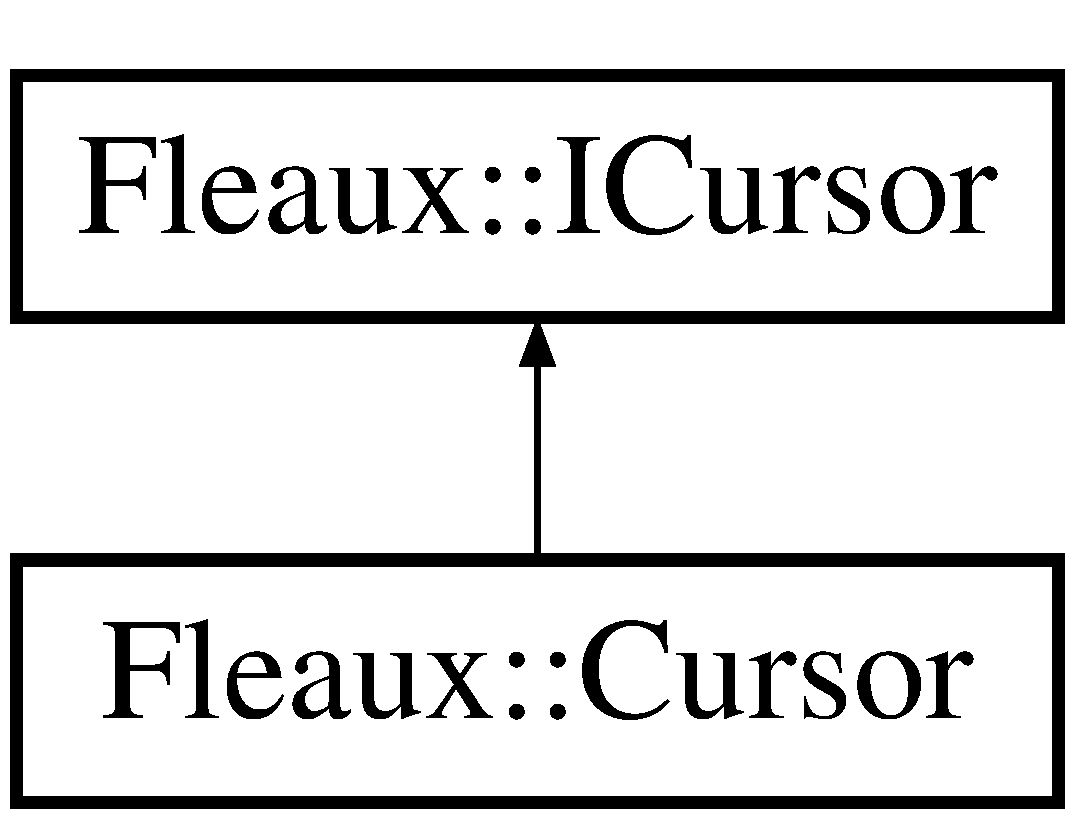
\includegraphics[height=2.000000cm]{classFleaux_1_1ICursor}
\end{center}
\end{figure}
\subsection*{Public Member Functions}
\begin{DoxyCompactItemize}
\item 
\hypertarget{classFleaux_1_1ICursor_a1293fc286aa66c2cfe1ba01096692073}{}virtual void {\bfseries insert} (const string \&input)=0\label{classFleaux_1_1ICursor_a1293fc286aa66c2cfe1ba01096692073}

\item 
\hypertarget{classFleaux_1_1ICursor_a0b236476cce265d4daf66a4dffc413b4}{}virtual void {\bfseries remove} (int length)=0\label{classFleaux_1_1ICursor_a0b236476cce265d4daf66a4dffc413b4}

\item 
\hypertarget{classFleaux_1_1ICursor_a0d6b32530ce9e5cdafd0d8e7e003b80f}{}virtual void {\bfseries replace} (int length, const string \&replacement)=0\label{classFleaux_1_1ICursor_a0d6b32530ce9e5cdafd0d8e7e003b80f}

\item 
\hypertarget{classFleaux_1_1ICursor_ae0aa625b46f91b0b46b5e582a2e1b0cf}{}virtual size\+\_\+t {\bfseries get\+Index} (void)=0\label{classFleaux_1_1ICursor_ae0aa625b46f91b0b46b5e582a2e1b0cf}

\item 
\hypertarget{classFleaux_1_1ICursor_a3aaabae93328864c7340dc71d9c9d4ca}{}virtual size\+\_\+t {\bfseries get\+X} (void)=0\label{classFleaux_1_1ICursor_a3aaabae93328864c7340dc71d9c9d4ca}

\item 
\hypertarget{classFleaux_1_1ICursor_ad0132bf4aad3ce917bf066eb2d0d2692}{}virtual size\+\_\+t {\bfseries get\+Y} (void)=0\label{classFleaux_1_1ICursor_ad0132bf4aad3ce917bf066eb2d0d2692}

\item 
\hypertarget{classFleaux_1_1ICursor_a77702f090f961857f53a06d9fb2f73b2}{}virtual void {\bfseries move} (int offset\+X, int offset\+Y)=0\label{classFleaux_1_1ICursor_a77702f090f961857f53a06d9fb2f73b2}

\end{DoxyCompactItemize}


The documentation for this class was generated from the following file\+:\begin{DoxyCompactItemize}
\item 
src/fleaux/headers/ieditor.\+hh\end{DoxyCompactItemize}

\hypertarget{classFleaux_1_1IEditor}{}\section{Fleaux\+:\+:I\+Editor Class Reference}
\label{classFleaux_1_1IEditor}\index{Fleaux\+::\+I\+Editor@{Fleaux\+::\+I\+Editor}}
Inheritance diagram for Fleaux\+:\+:I\+Editor\+:\begin{figure}[H]
\begin{center}
\leavevmode
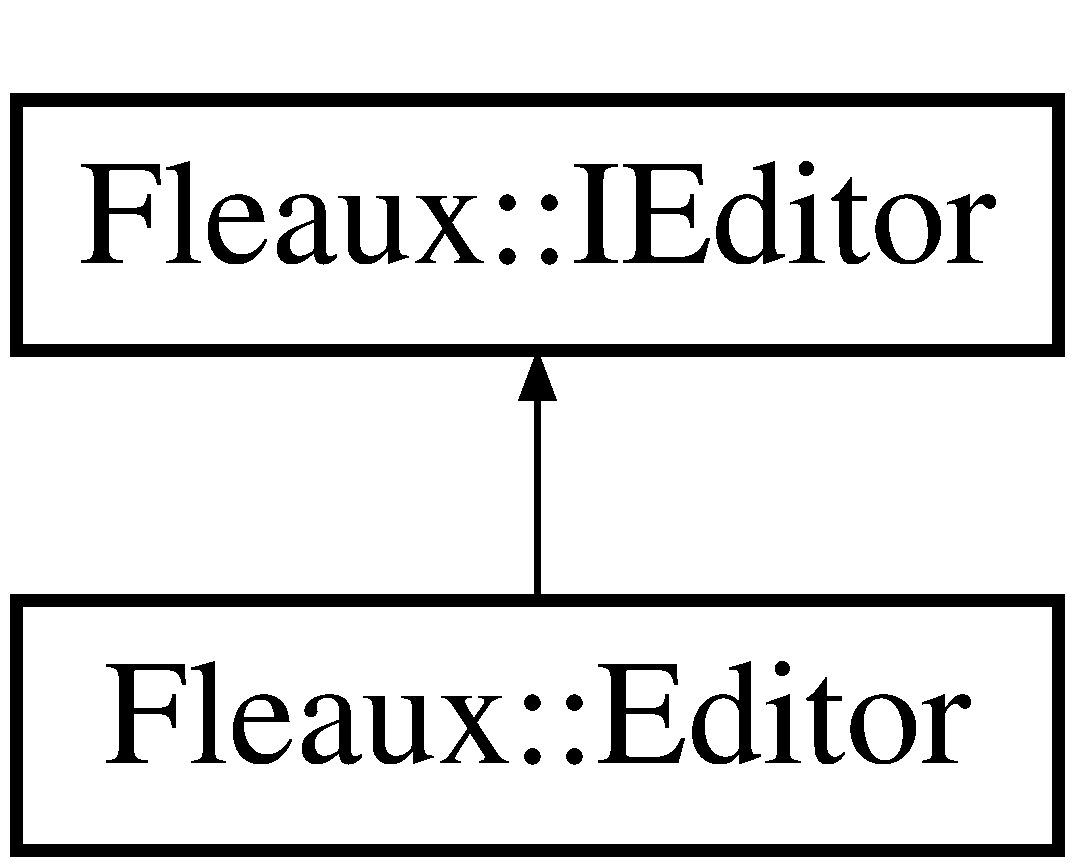
\includegraphics[height=2.000000cm]{classFleaux_1_1IEditor}
\end{center}
\end{figure}
\subsection*{Public Member Functions}
\begin{DoxyCompactItemize}
\item 
\hypertarget{classFleaux_1_1IEditor_af90c1eec6bebbc836bb249b21171ea5d}{}virtual void {\bfseries read\+From\+File} (const string \&path)=0\label{classFleaux_1_1IEditor_af90c1eec6bebbc836bb249b21171ea5d}

\item 
\hypertarget{classFleaux_1_1IEditor_a4ff158a235ed9991af521f08e7cef58e}{}virtual void {\bfseries write\+To\+File} (const string \&path)=0\label{classFleaux_1_1IEditor_a4ff158a235ed9991af521f08e7cef58e}

\item 
\hypertarget{classFleaux_1_1IEditor_adbed8262a17bf6e261026d3f4d15486e}{}virtual \hyperlink{classFleaux_1_1ICursor}{I\+Cursor} $\ast$ {\bfseries get\+Cursor} (void)=0\label{classFleaux_1_1IEditor_adbed8262a17bf6e261026d3f4d15486e}

\end{DoxyCompactItemize}


The documentation for this class was generated from the following file\+:\begin{DoxyCompactItemize}
\item 
src/fleaux/headers/ieditor.\+hh\end{DoxyCompactItemize}

%--- End generated contents ---

% Index
\backmatter
\newpage
\phantomsection
\clearemptydoublepage
\addcontentsline{toc}{chapter}{Index}
\printindex

\end{document}
